\documentclass[12pt,a4paper]{article}

\usepackage[T1]{fontenc}
\usepackage[utf8]{inputenc}
\usepackage{csquotes}
\usepackage{newtxtext,newtxmath}
\usepackage{amsmath}
\usepackage{url}
\usepackage{graphicx}
\graphicspath{{figures/}}
\usepackage{float}
\usepackage{enumitem}
\usepackage{setspace}
\usepackage{geometry}
\usepackage{array}
\usepackage{pdflscape}
\usepackage{afterpage}
\usepackage{longtable}
\usepackage{placeins}
\usepackage{booktabs}
\usepackage[backend=biber,style=apa,sortcites=true,sorting=nyt,maxcitenames=2,uniquelist=false]{biblatex}
\DeclareLanguageMapping{english}{english-apa}
\addbibresource{references.bib}

\geometry{margin=2.5cm}
\doublespacing

\title{Enhancing Socio-Emotional Functioning of Adults with Disabilities:\\
Evaluation of an Experiential Intervention in a Day Care Facility}

% Author information is provided on the separate title page (double-anonymous peer review)

\date{}

\begin{document}

\maketitle

% ---------------------------------------------------------------
% ABSTRACT (structured)
% ---------------------------------------------------------------
\begin{abstract}
\noindent\textbf{Background:} Adults with intellectual and psychosocial disabilities have limited access to structured socio-emotional development programs in community care settings.

\noindent\textbf{Method:} A three-phase longitudinal design evaluated an arts-based socio-emotional program over three months in a Day Care Center ($n = 30$ adults, 80\% with a documented intellectual disability). Data were collected from beneficiary self-reports, trainer/educator assessments, and independent observer ratings using an 11-item Likert-scale instrument developed for the study.

\noindent\textbf{Results:} Significant improvements were observed across all evaluator sources. Beneficiary self-reports showed the largest effect ($d = 2.45$, $p < .001$), followed by trainers/educators ($d = 1.62$) and the independent observer ($d = 1.40$). Friedman tests confirmed significant longitudinal change across phases ($p < .001$).

\noindent\textbf{Conclusions:} Participation in a holistic experiential program was associated with notable improvements in emotion recognition, cooperation, group participation, and well-being among adults with intellectual and developmental disabilities in a Day Care setting. In the absence of a control group, these findings are preliminary but consistent across sources.
\end{abstract}

% ---------------------------------------------------------------
% LAY SUMMARY (3–4 bullet points)
% ---------------------------------------------------------------
\subsection*{Lay Summary}
\begin{itemize}
    \item Adults with intellectual and psychosocial disabilities attending a Day Care Center showed substantial improvements in socio-emotional skills---including emotion recognition, cooperation, and group participation---following a structured arts-based intervention.
    \item Improvements were consistently confirmed by three independent sources: the participants themselves, their trainers/educators, and an independent observer, strengthening the reliability of the findings.
    \item The intervention combined theatre, music, movement, ceramics, and narrative dialogue within a group-based format, offering a replicable and documented model for Day Care services supporting adults with disabilities.
    \item These findings support the integration of arts-based socio-emotional programs in Day Care settings as a pathway to enhanced emotional well-being, social inclusion, and quality of life for adults with disabilities.
\end{itemize}

\noindent\textbf{Keywords:} social-emotional learning; emotional intelligence; adults with disabilities; day care centers; group interventions; social inclusion; program evaluation

\section{Introduction}

Socio-emotional functioning constitutes a fundamental factor for the quality of life, empowerment, and social inclusion of persons with disabilities. Contemporary international literature recognizes that skills such as emotion recognition and expression, self-regulation, social awareness, empathy, and cooperation form a critical basis for participation in social, educational, and occupational contexts \parencite{casel2020,weissberg2015}. Emotional intelligence, as conceptualized by \textcite{goleman1995}, has also been identified as an important factor associated with well-being, resilience, and successful interpersonal relationships.

In the context of Day Care Centers (DCCs)\footnote{Day Care Centers are facilities providing organized daily care, education, social inclusion, and support services for adults with disabilities, operating within a legislative framework for disability services. Their objectives include enhancing autonomy, developing skills, promoting social participation, and relieving families, through individualized and group-based psychosocial and functional support programs.}, which provide structured daily support to adults with intellectual and psychosocial difficulties, the development of socio-emotional skills becomes particularly important. DCCs combine education, care, psychosocial support, and social inclusion, offering beneficiaries opportunities to develop stable social relationships, autonomy-related skills, and self-esteem \parencite{westmore2024}.

The theoretical basis of this study draws on socio-cultural, group-based, and relational approaches to learning and development. Vygotsky's theory emphasizes the role of social interaction as a driving force of learning \parencite{vygotsky1978}, supporting the need for interventions that promote cooperation, dialogue, and experiential engagement. Similarly, \textcite{yalom2005} highlight the therapeutic value of group processes, particularly in enhancing empathy, authentic expression, and emotional connectedness among participants. These principles are especially relevant for adults with disabilities, whose socio-emotional development is strongly influenced by their participation in safe and supportive social environments \parencite{shogren2017}.

The effectiveness of group interventions cannot be explained solely by the content of the activities, but also by group dynamics and the quality of interpersonal relationships developed within the group. Research on group therapy indicates that group cohesion is a consistent, moderate predictor of positive therapeutic outcomes \parencite{burlingame2011}. Cohesion is associated with feelings of safety, trust, and acceptance, which facilitate authentic emotional expression and active participation. Moreover, the therapeutic relationship has been identified as a critical factor of change across different intervention models \parencite{norcross2018,wampold2015}.

Emotional safety and the experience of acceptance are essential preconditions for the development of socio-emotional skills. Attachment theory suggests that a secure base enables individuals to explore, express themselves, and experiment with new behaviors without fear of rejection \parencite{bowlby1988}. In group contexts, this secure-base function may operate collectively, allowing the group to function as a space of emotional containment and experiential processing. Interpersonal neurobiology further supports the idea that emotional regulation develops through relationships and social interaction \parencite{siegel2012,schore2012}.

Despite the theoretical and empirical importance of socio-emotional development, important gaps remain in the literature. Most studies focus on children and adolescents in school contexts \parencite{durlak2011,humphrey2013,oberle2019}, whereas research concerning adults in day care settings remains limited. Existing studies on community participation among adults with intellectual disabilities document both its importance and its persistent limitations \parencite{hall2009,verdonschot2009}; however, they rarely combine a multi-phase longitudinal design with multiple sources of evaluation, such as beneficiaries, trainers, and independent observers.

The present study addresses these gaps by systematically evaluating a holistic, experiential socio-emotional empowerment program implemented in a DCC setting. Its contribution is fivefold. First, it examines a structured intervention in a day care context, which remains underexplored in the literature. Second, it uses three independent sources of evaluation: beneficiary self-reports, trainer/educator assessments, and independent observer ratings. Third, it adopts a three-phase longitudinal design, allowing the analysis of change over time. Fourth, it combines statistical significance testing with effect-size estimation and trajectory analysis. Fifth, it connects theory and practice by integrating Social and Emotional Learning (SEL), emotional intelligence, socio-cultural learning theory, and group therapeutic factors.

A further contribution of this study lies in the arts-based nature of the intervention. The program, entitled ``The Universe Within Us,'' included experiential practices such as theatrical expression, music, movement, symbolic object creation, and narrative activities. These practices aimed to cultivate SEL-related skills through symbolic, embodied, and interpersonal learning. Arts-based approaches have been described as particularly valuable for groups with complex support needs, as they allow expression, participation, and meaning-making beyond purely verbal modes of communication \parencite{leavy2015,stickley2018}.

Based on the international literature and the theoretical framework of SEL, the present study adopts a conceptual model organized around three interrelated dimensions: social interaction and communication skills, socio-emotional well-being and emotional regulation, and active participation within the group. The model assumes that a systematic, experiential, and group-based intervention can activate mechanisms of change such as safe emotional expression, group cohesion, social reinforcement, and gradual internalization of socio-emotional skills. These mechanisms are expected to lead to improvements in the socio-emotional functioning of the beneficiaries.

Accordingly, the study formulates the following hypotheses:

\begin{enumerate}[label=\arabic*.]
    \item The intervention will be associated with statistically significant improvement in socio-emotional functioning between Phase A and Phase C.
    \item Improvement will be observed across all three independent sources of evaluation: beneficiaries, trainers/educators, and the independent observer.
    \item The trajectory of change will be progressive and statistically significant across consecutive phases.
\end{enumerate}

\begin{figure}[!t]
\centering
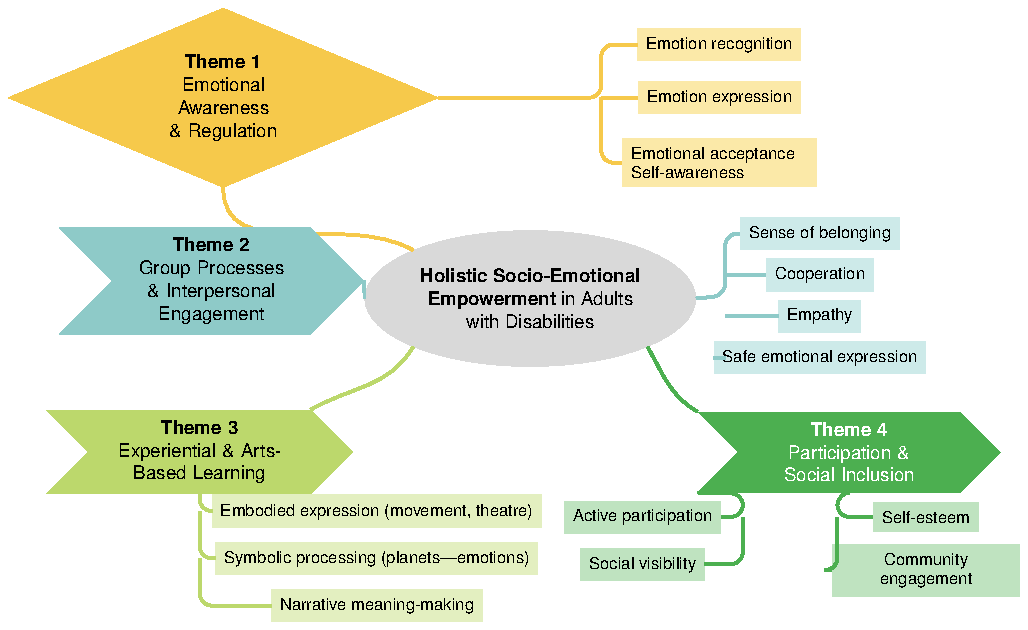
\includegraphics[width=\textwidth]{conceptual_model.pdf}
\caption{Conceptual model of the intervention and mechanisms of change.}
\label{fig:conceptual_model}
\end{figure}

Figure~\ref{fig:conceptual_model} presents the conceptual model of the intervention and the proposed mechanisms of empowerment.


\section{Background}

Earlier approaches in the field often focused primarily on functional training or behavioral compliance \parencite{emerson2001}, with limited attention to the emotional, relational, and participatory dimensions of adult life with disability. These approaches, while effective in addressing specific behavioral targets, have been criticized for their narrow scope, their tendency to treat adults with disabilities as passive recipients of intervention, and their failure to address broader psychosocial needs such as belonging, identity, and self-determination \parencite{mcnaughton2025,witwer2022}. More recent research has therefore shifted toward interventions that promote self-awareness, emotional regulation, belonging, participation, and inclusion in community and group contexts, recognizing that socio-emotional competencies are not peripheral but central to quality of life and meaningful social participation.

\textcite{giummarra2022} provide a broad synthesis of interventions targeting social and community participation among adults with autism spectrum disorder, intellectual disability, and psychosocial disability. Their findings suggest that experiential participation, safe social contexts, and stable group involvement are associated with improvements in social functioning, self-esteem, and emotional well-being. Nevertheless, the review relies exclusively on secondary synthesis without primary data collection, does not employ standardized outcome measures across studies, and lacks longitudinal follow-up, limiting the comparability and generalizability of findings across different service settings.

\textcite{littlewood2018} examined emotion regulation strategies used by adults with mild intellectual disability in everyday social interactions. Their findings indicate that participants often develop informal and experience-based regulation strategies through social interaction. This supports the need for interventions embedded in real social contexts rather than isolated instructional settings. However, the qualitative design of the study precludes quantitative effectiveness measurement, and the exclusive focus on mild intellectual disability limits applicability to populations with more complex support needs.

\textcite{jacob2022} systematically reviewed interventions aiming to improve social skills in individuals with intellectual disability. The reviewed strategies included peer tutoring\footnote{An educational practice in which an individual is supported in learning or developing skills by a peer with similar characteristics or experiences, relying on social interaction and peer reinforcement.}, video modelling\footnote{A technique in which the individual observes video-recorded behavioral models and is prompted to replicate them, particularly effective as it reduces language demands and strengthens observational learning.}, and play-based emotional regulation interventions. Although many interventions showed positive outcomes, the authors highlighted the lack of integrated programs combining multiple SEL-related skills within a longitudinal evaluation design. A further limitation concerns the diversity of measurement instruments across reviewed studies, which impedes the synthesis of comparable effect sizes and the identification of common mechanisms of change.

In intervention research, \textcite{vanutelli2023} conducted a pilot study of an emotional skills training program for eight adults with intellectual disability, delivered during the COVID-19 period, and reported gains in emotion recognition and expression on pre--post assessment. Their work supports the feasibility of structured, experiential emotional training with adults with intellectual disability. Its primary limitations are the very small sample, the absence of a control condition, and reliance on a single evaluator perspective, which restrict generalizability and preclude triangulation across sources.

Recent work has also emphasized the heterogeneity of psychological interventions for adults with intellectual disability. \textcite{witwer2022} argues that many interventions lack a clear theoretical framework and systematic evaluation, making it difficult to identify which components drive positive outcomes. Similarly, \textcite{mcnaughton2025} emphasize that meaningful social participation among adults with developmental disabilities requires interventions that strengthen voice, agency, participation, and belonging, rather than focusing only on isolated skill acquisition. Both contributions, however, remain theoretical in nature and do not provide empirical data on intervention effectiveness, which limits their direct applicability to evidence-based practice.

At the cognitive level, \textcite{okafor2025} link cognitive processing speed with emotion regulation in adults with intellectual disability. This finding suggests that interventions relying exclusively on verbal processing may be limited. It also strengthens the rationale for experiential and multimodal interventions that use bodily, symbolic, emotional, and interpersonal forms of engagement. A notable challenge in this line of research, however, is the absence of an intervention component: the study establishes a neuropsychological association but does not test whether targeted programs can modify these processes in applied settings.

From a theoretical perspective, \textcite{sappok2022} propose a social neuroscience framework for understanding socio-emotional development in individuals with intellectual disability. Their work emphasizes that emotional processing and social behavior are shaped through ongoing interaction with the environment. This framework is directly relevant to group-based and community-embedded interventions. However, as a theoretical analysis without empirical intervention data, the framework requires further validation through applied studies that test its predictions in real-world care contexts.

Finally, \textcite{parsakia2024} examined experiences of community participation among adults with intellectual disability. Their findings indicate that participation, acceptance, and emotional safety are central indicators of successful inclusion, often more important than isolated functional skills. Despite the richness of the qualitative data, the study does not include quantitative measures of socio-emotional outcomes, nor does it evaluate a structured intervention, leaving open the question of how these experiential conditions can be systematically cultivated in day care settings.

Overall, the literature suggests that interventions targeting socio-emotional functioning in adults with disabilities are more effective when they are experiential, multimodal, socially embedded, and evaluated through longitudinal and multi-source designs. However, there remains a clear gap in structured programs that combine these characteristics within day care settings. The present intervention, entitled ``The Universe Within Us,'' responds to this gap by adopting a holistic, arts-based, community-oriented SEL approach for adults with disabilities in a DCC context.
Table~\ref{tab:literature_comparison} summarizes selected studies and highlights the differentiation of the present research.

\afterpage{%
\begin{landscape}
\singlespacing
\footnotesize
\setlength{\LTcapwidth}{\linewidth}
\begin{longtable}{p{2.5cm} p{3.0cm} p{3.8cm} p{3.0cm} p{2.8cm} p{3.0cm} p{3.8cm}}
\caption{Categorization of Related Studies and Differentiation of the Present Research}
\label{tab:literature_comparison}\\
\hline
\textbf{Study} & \textbf{Population} & \textbf{Intervention / Focus} & \textbf{Theoretical Framework} & \textbf{Design} & \textbf{Evaluation} & \textbf{Main Limitations} \\
\hline
\endfirsthead
\multicolumn{7}{c}{\tablename~\thetable{} \textit{-- continued from previous page}}\\
\hline
\textbf{Study} & \textbf{Population} & \textbf{Intervention / Focus} & \textbf{Theoretical Framework} & \textbf{Design} & \textbf{Evaluation} & \textbf{Main Limitations} \\
\hline
\endhead
\hline
\multicolumn{7}{r}{\footnotesize\textit{Continued on next page}}\\
\endfoot
\hline
\endlastfoot
\textcite{giummarra2022} & Adults ($\geq$18 yrs) with intellectual disabilities, autism spectrum disorder, and psychosocial disabilities; 57 reviews covering 522 studies & Social and community participation & Participatory inclusion and well-being & Umbrella review & Secondary synthesis & No primary data; heterogeneous outcome measures; limited longitudinal follow-up \\
\textcite{littlewood2018} & $n=11$ adults with mild intellectual disabilities; age not reported & Emotion regulation in everyday life & Experiential approach & Qualitative study & Semi-structured interviews & No quantitative effectiveness measurement; limited to mild intellectual disabilities only \\
\textcite{jacob2022} & Children and adolescents with intellectual disabilities across 10 studies ($n$ ranging from 3 to 296; age range: 7--19 yrs) & Social skills interventions & Behavioral and social theories & Systematic review & Diverse instruments & Heterogeneous measures; lack of unified theoretical framework; limited adult representation \\
\textcite{vanutelli2023} & $n=8$ adults with intellectual disabilities; emotional skills training during COVID-19 & Emotional competencies training & Educational and experiential approach & Pilot intervention study & Pre--post assessment (quantitative and qualitative) & Very small sample; limited generalizability; no control group \\
\textcite{witwer2022} & N/A -- theoretical analysis; adults with intellectual disabilities (reviewed literature) & Psychological interventions & Diverse frameworks & Scoping review & Secondary analysis & No primary sample; lack of comparable evaluations across interventions \\
\textcite{mcnaughton2025} & N/A -- theoretical article; adults with developmental disabilities & Social participation and agency & Participatory models & Theoretical article & Not applicable & No empirical data; findings not directly testable without primary research \\
\textcite{okafor2025} & Adults with intellectual disabilities; neuropsychological assessment sample & Cognitive processing speed and emotion regulation & Neurocognitive approach & Quantitative study & Neuropsychological tests & No intervention component; associational findings only \\
\textcite{sappok2022} & N/A -- theoretical analysis; people with intellectual disabilities (conceptual framework) & Socio-emotional development & Social neuroscience & Theoretical analysis & Not applicable & No primary sample; framework requires empirical validation in applied settings \\
\textcite{parsakia2024} & Adults with intellectual disabilities; qualitative community sample & Community participation & Phenomenological approach & Qualitative study & Thematic analysis & No quantitative outcome measures; no structured intervention evaluated \\
Present study & $n=30$ adults with intellectual and psychosocial disabilities in a DCC (80\% with documented intellectual disability; mean age 34.4 yrs, $SD=10.6$; complete longitudinal sample) & Holistic arts-based SEL intervention & SEL, EI, Vygotsky, Yalom & Three-phase longitudinal design & Three-source evaluation (self-report, educators, independent observer) and effect sizes & No control group; single-site study; tool not formally validated \\
\end{longtable}
\end{landscape}
}

\section{Method}

\subsection{Study Setting and Participants}

The study was conducted at a Day Care Center in southern Greece providing educational and psychosocial programs for adults with intellectual and developmental disabilities. A total of 30 adult beneficiaries participated (20 men and 10 women; age range 20--55 years, $M = 34.4$, $SD = 10.6$). All participants attended the daily program systematically and had the capacity, or supported capacity, to provide informed consent; where applicable, consent was also obtained from legal guardians.

Participant characteristics, drawn from official disability certification records, are summarized in Table~\ref{tab:demographics}. Twenty-four participants (80.0\%) had a documented diagnosis of intellectual disability (mild: $n = 5$; moderate: $n = 11$; severe: $n = 6$; severity not specified in the record: $n = 2$). The remaining six participants had primary diagnoses of psychotic disorder ($n = 4$), autism spectrum disorder with cognitive functioning above the intellectual disability threshold ($n = 1$), or cerebral palsy ($n = 1$). Co-occurring conditions were common: nine participants had a psychiatric diagnosis (psychotic disorder or schizophrenia), five had autism spectrum disorder, and six had physical or sensory impairments (motor disability, visual impairment, or epilepsy). The sample therefore reflects the heterogeneous population typically served by Greek day care centers, where intellectual, developmental, and psychosocial disabilities frequently co-occur. No formal measure of adaptive behavior was administered; this is acknowledged as a limitation.

\begin{table}[!t]
\caption{Demographic and Clinical Characteristics of Participants ($N = 30$)}
\label{tab:demographics}
\centering
\begin{tabular}{lc}
\hline
\textbf{Characteristic} & $\boldsymbol{n}$ \textbf{(\%)} \\
\hline
Male & 20 (66.7) \\
Female & 10 (33.3) \\
Age, years, $M$ ($SD$) & 34.4 (10.6) \\
Age range, years & 20--55 \\
\hline
\multicolumn{2}{l}{\textit{Intellectual disability (documented)}} \\
\quad Mild & 5 (16.7) \\
\quad Moderate & 11 (36.7) \\
\quad Severe & 6 (20.0) \\
\quad Severity not specified & 2 (6.7) \\
\quad Not documented & 6 (20.0) \\
\hline
\multicolumn{2}{l}{\textit{Co-occurring conditions}} \\
\quad Psychotic disorder / schizophrenia & 9 (30.0) \\
\quad Autism spectrum disorder & 5 (16.7) \\
\quad Physical / sensory / neurological & 6 (20.0) \\
\quad None recorded & 11 (36.7) \\
\hline
\multicolumn{2}{p{0.85\linewidth}}{\footnotesize\textit{Note.} Categories of co-occurring conditions are not mutually exclusive. Six participants without a documented intellectual disability had primary diagnoses of psychotic disorder ($n = 4$), autism spectrum disorder ($n = 1$), or cerebral palsy ($n = 1$).} \\
\end{tabular}
\end{table}

Self-report data were complete for all 30 participants across the three measurement phases. Trainer ratings were obtained from two educators who worked daily with the beneficiaries, and one independent observer with experience in special education rated all participants. The electronic export of the rating platform did not contain trainer ratings for 18 and observer ratings for 12 of the 90 participant--phase records per source (four participants had no trainer or observer record in any phase), and contained only one of the two trainer ratings for 17 further records. These ratings were supplied by the facility in a supplementary data file after the export had been produced and were merged with the export at the level of individual ratings, before any aggregation. After merging, ratings were available from all three sources for all 30 participants in all three phases. For each participant and phase, the two trainer ratings were averaged item-wise to yield a single trainer-based score; for two records only one educator's rating was available and was used as such. Where a rater had submitted the same assessment twice, the first submission was retained. No values were imputed, and all analyses were conducted on $n = 30$ for each evaluator category.

\subsection{Researcher Positionality}

The relationship between the authors and the study setting is stated transparently. The first author coordinates the digital infrastructure of the Day Care Center and was responsible for data management and statistical analysis; he had no role in designing or delivering the intervention and did not rate any participant. The second and third authors are members of the facility's staff (an educator and the psychologist-psychotherapist, respectively) who designed and facilitated the intervention; neither provided trainer or observer ratings. The fourth author, an academic supervisor external to the facility, oversaw the research design and analysis. Trainer ratings were provided by two educators employed at the facility who worked with the beneficiaries daily but were not involved in authorship. The independent observer was an external special education professional with no employment relationship to the facility and no prior contact with the participants.

This configuration carries an inherent risk of positive expectancy among program-affiliated raters. We sought to mitigate this risk in three ways: trainer scores were averaged across both raters; an external, unaffiliated observer provided an independent assessment; and convergence across the three sources was examined explicitly. Nevertheless, the trainers were not blinded to the aims of the program, and the facility's institutional interest in demonstrating program value is acknowledged as a potential source of bias. The independent observer's ratings, which showed the most conservative absolute scores and the smallest, though still large, effect size, offer the least conflicted evidence of change.

\subsection{Research Design}

The study followed a three-phase longitudinal design over a period of three months. Phase A was conducted at the beginning of the program (baseline), Phase B at approximately the midpoint of the intervention (around six weeks into implementation), and Phase C after the completion of the intervention at the end of the third month. These three consecutive measurements enabled the assessment of both immediate and progressive effects of the intervention, while Phase B served as an intermediate observation point.

\subsection{Intervention Description}

The intervention was implemented over a period of three months,
comprising approximately 36 structured sessions in total, with
three sessions per week, each lasting between 45 and 60 minutes.
Sessions were conducted in small groups of 6 to 10 participants
and followed a consistent structure: an opening warm-up activity,
a core experiential task (artistic, theatrical, or movement-based),
and a closing reflective dialogue. The weekly schedule remained
stable throughout the implementation period to provide predictability
and emotional safety. The psychologist-psychotherapist facilitating
the sessions held a postgraduate qualification in psychotherapy and
had prior experience working with adults with intellectual and
psychosocial disabilities. No formal fidelity checklist was applied;
however, session consistency was maintained through a fixed
activity protocol developed prior to implementation.

The intervention was holistic and experiential in nature. It was organized around activities involving emotion recognition and expression, empathy exercises, collaborative tasks, and group processes. The intervention was theoretically informed by SEL \parencite{casel2020}, emotional intelligence \parencite{goleman1995}, Vygotsky's socio-cultural theory \parencite{vygotsky1978}, and Yalom's therapeutic factors of group work \parencite{yalom2005}.

The structure of the program remained stable throughout the implementation period. Weekly activities were conducted in small groups and included goal setting, repeated experiential patterns, and structured opportunities for social interaction. The intervention was implemented with the continuous presence of a psychologist-psychotherapist, who supported the emotional safety of the group, facilitated expression, and strengthened interpersonal understanding among participants. This role extended beyond instructional guidance and contributed to the development of therapeutic alliance and group cohesion, both of which are recognized as important mechanisms of change \parencite{norcross2018,burlingame2011}.

The intervention was embedded in the arts-based experiential program entitled ``The Universe Within Us.'' The program aimed to enhance the recognition, expression, and acceptance of emotions through multimodal artistic processes. It included:

\begin{itemize}
    \item theatrical exercises and role-play activities;
    \item movement and bodily expression;
    \item music and original song composition;
    \item ceramics and visual creation;
    \item construction of ``emotion-planets'';
    \item group dialogue and empathy-based discussions.
\end{itemize}

Each beneficiary participated in the creation of symbolic planets, each representing a different emotion. This process promoted symbolism, self-expression, and embodied emotional processing, in line with principles of arts-based interventions \parencite{malchiodi2020,goldstein2017,hinz2009}. The program culminated in a music-theatre performance at a public amphitheatre, with the participation of kindergartens and primary schools. This public presentation aimed to enhance self-esteem, social visibility, and community inclusion, consistent with the international framework of community arts inclusion \parencite{nicholson2005,white2013}.

\subsection{Assessment Instrument}

Socio-emotional functioning was assessed using a structured instrument consisting of 11 indicators rated on a five-point Likert scale, ranging from 1 (not at all) to 5 (very much). The instrument was designed to assess core SEL-related dimensions, including:

\begin{enumerate}
    \item emotion expression;
    \item emotion recognition;
    \item emotion acceptance;
    \item self-awareness;
    \item sense of belonging to the group;
    \item cooperation;
    \item creativity and enjoyment;
    \item active participation;
    \item well-being and self-esteem;
    \item overall evaluation;
    \item willingness to participate and to recommend the program to others.
\end{enumerate}

The first ten indicators were derived from the SEL framework; the eleventh captures behavioral intention and program acceptability rather than a socio-emotional competency per se, and was retained in the composite score because it was administered to all evaluator categories in parallel form. The indicators do not map one-to-one onto the five CASEL competency domains: several indicators (emotion expression, recognition, acceptance, and self-awareness) jointly operationalize self-awareness and self-management, whereas social awareness, relationship skills, and responsible decision-making are represented by fewer items each.

The same indicator system was adapted into three distinct formulations in order to capture different temporal perspectives. Phase A reflected the participant's general self-perception before the intervention. Phase B assessed the experience of the specific session and intermediate progress. Phase C assessed the perceived overall effect of the program. This threefold structure strengthened content validity and allowed the measurement of both general characteristics and intervention-related change.

The instrument demonstrated acceptable to high internal consistency in most evaluator categories and phases, with Cronbach's alpha values ranging from 0.79 to 0.96 (Table~\ref{tab:cronbach}); the lower value for beneficiary self-reports in Phase C ($\alpha = 0.69$) is consistent with the restricted variance of scores in that phase. For trainers/educators, alpha was computed on the item-wise mean of the two educators' ratings per participant.

\begin{table}[!t]
\caption{Internal Consistency (Cronbach's $\alpha$) of the Assessment Instrument by Evaluator Category and Phase ($n = 30$)}
\label{tab:cronbach}
\centering
\begin{tabular}{lccc}
\hline
\textbf{Evaluator Category} & \textbf{Phase A} & \textbf{Phase B} & \textbf{Phase C} \\
\hline
Beneficiaries & 0.90 & 0.95 & 0.69 \\
Trainers/Educators & 0.95 & 0.96 & 0.95 \\
Independent observer & 0.82 & 0.87 & 0.79 \\
\hline
\end{tabular}
\end{table}

The assessment instrument was developed specifically for this study
by the lead researcher and psychologist-psychotherapist responsible
for the intervention, drawing on the five core competency domains
of the CASEL SEL framework \parencite{casel2020} and established
theoretical frameworks of emotional intelligence \parencite{goleman1995}.
Item generation followed a content-driven approach: each indicator
was mapped onto a specific SEL dimension (emotion recognition,
self-regulation, cooperation, group belonging, and well-being),
and linguistic accessibility was prioritized to accommodate the
cognitive and communicative characteristics of the target population.
The instrument was reviewed by two special education professionals
prior to administration and minor wording adjustments were made
based on their feedback. No formal pilot study was conducted prior
to the main data collection. Internal consistency served as the
primary reliability indicator, while convergence across three
independent evaluator sources provided supplementary support for
content validity. Nevertheless, the absence of formal psychometric
validation (factor analysis, convergent validity) remains a
limitation that future research should address.

\subsection{Statistical Analysis}

The statistical analysis combined descriptive and inferential techniques. First, means, standard deviations, and 95\% confidence intervals were calculated for each phase and evaluator category. To examine the effectiveness of the intervention, paired-sample $t$-tests were applied by comparing Phase A and Phase C scores for each evaluator category \parencite{student1908}. Effect sizes were calculated using Cohen's $d$ with corresponding confidence intervals \parencite{cohen1988}.

The longitudinal trajectory of scores across the three phases was examined graphically and statistically. Boxplots and violin plots were used to visualize the distribution of values before and after the intervention, while a trajectory plot was used to illustrate the evolution of mean scores across phases.

All analyses were conducted using Python 3.12, with the pandas, SciPy, and Matplotlib libraries. The level of statistical significance was set at $\alpha=.05$. Prior to the application of parametric tests, the distribution of the Phase C $-$ Phase A difference scores was examined using the Shapiro--Wilk test. Because a non-significant Shapiro--Wilk test does not establish normality, particularly with $n = 30$, the Wilcoxon signed-rank test was additionally applied to each evaluator category as a non-parametric check.

For the extended analysis of change across the three phases, the Friedman test was used. Pairwise comparisons between Phase A--Phase B, Phase B--Phase C, and Phase A--Phase C were conducted using Bonferroni-corrected paired $t$-tests, with an adjusted significance threshold of $\alpha_{\mathrm{adj}}=.017$. Given the sample size and the applied nature of the study, these tests were preferred over more complex mixed-effects models, which require larger samples for reliable estimation.

The analysis code is openly available at a public repository (URL blinded for review).


\section{Results}

\subsection{Descriptive Statistics and Distributional Patterns}

Descriptive statistics for socio-emotional functioning scores across phases and evaluator categories are presented in Table~\ref{tab:descriptive_statistics}. A consistent increase in mean scores was observed from Phase A to Phase C across all evaluator categories, indicating progressive improvement during the intervention. The relatively narrow 95\% confidence intervals suggest stability in the estimates.

\begin{table}[!t]
\caption{Descriptive Statistics of Socio-Emotional Functioning Scores by Phase and Evaluator Category}
\label{tab:descriptive_statistics}
\centering
\begin{tabular}{llcccc}
\hline
\textbf{Evaluator} & \textbf{Phase} & \textbf{Mean} & \textbf{SD} & \textbf{95\% CI Lower} & \textbf{95\% CI Upper} \\
\hline
Beneficiaries & A & 3.24 & 0.62 & 3.02 & 3.46 \\
Beneficiaries & B & 3.71 & 0.62 & 3.49 & 3.93 \\
Beneficiaries & C & 4.75 & 0.18 & 4.69 & 4.82 \\
Trainers/Educators & A & 2.68 & 0.56 & 2.48 & 2.88 \\
Trainers/Educators & B & 3.01 & 0.55 & 2.82 & 3.21 \\
Trainers/Educators & C & 3.30 & 0.46 & 3.13 & 3.46 \\
Independent observer & A & 2.18 & 0.33 & 2.06 & 2.30 \\
Independent observer & B & 2.45 & 0.32 & 2.34 & 2.57 \\
Independent observer & C & 2.58 & 0.28 & 2.48 & 2.68 \\
\hline
\end{tabular}
\end{table}


The graphical representation of scores before and after the intervention is presented in Figures~\ref{fig:boxplot} and~\ref{fig:violin}. The boxplots indicate a clear and systematic upward shift in central tendency from Phase A to Phase C across all evaluator categories. For beneficiaries, the median increased substantially, while the interquartile range decreased, suggesting greater homogeneity in socio-emotional functioning after the completion of the program.

For trainers/educators, the boxplots also reveal a steady increase in median scores across the three phases without outlying values; the interquartile range did not narrow, indicating that the improvement was accompanied by continued between-participant variability in educators' evaluations. The independent observer showed a similar upward pattern, with Phase C scores occupying a higher area of the scale compared with Phase A. Overall, the boxplots suggest that improvement was not limited to mean scores, but affected the broader distribution of values.

\begin{figure}[!t]
\centering
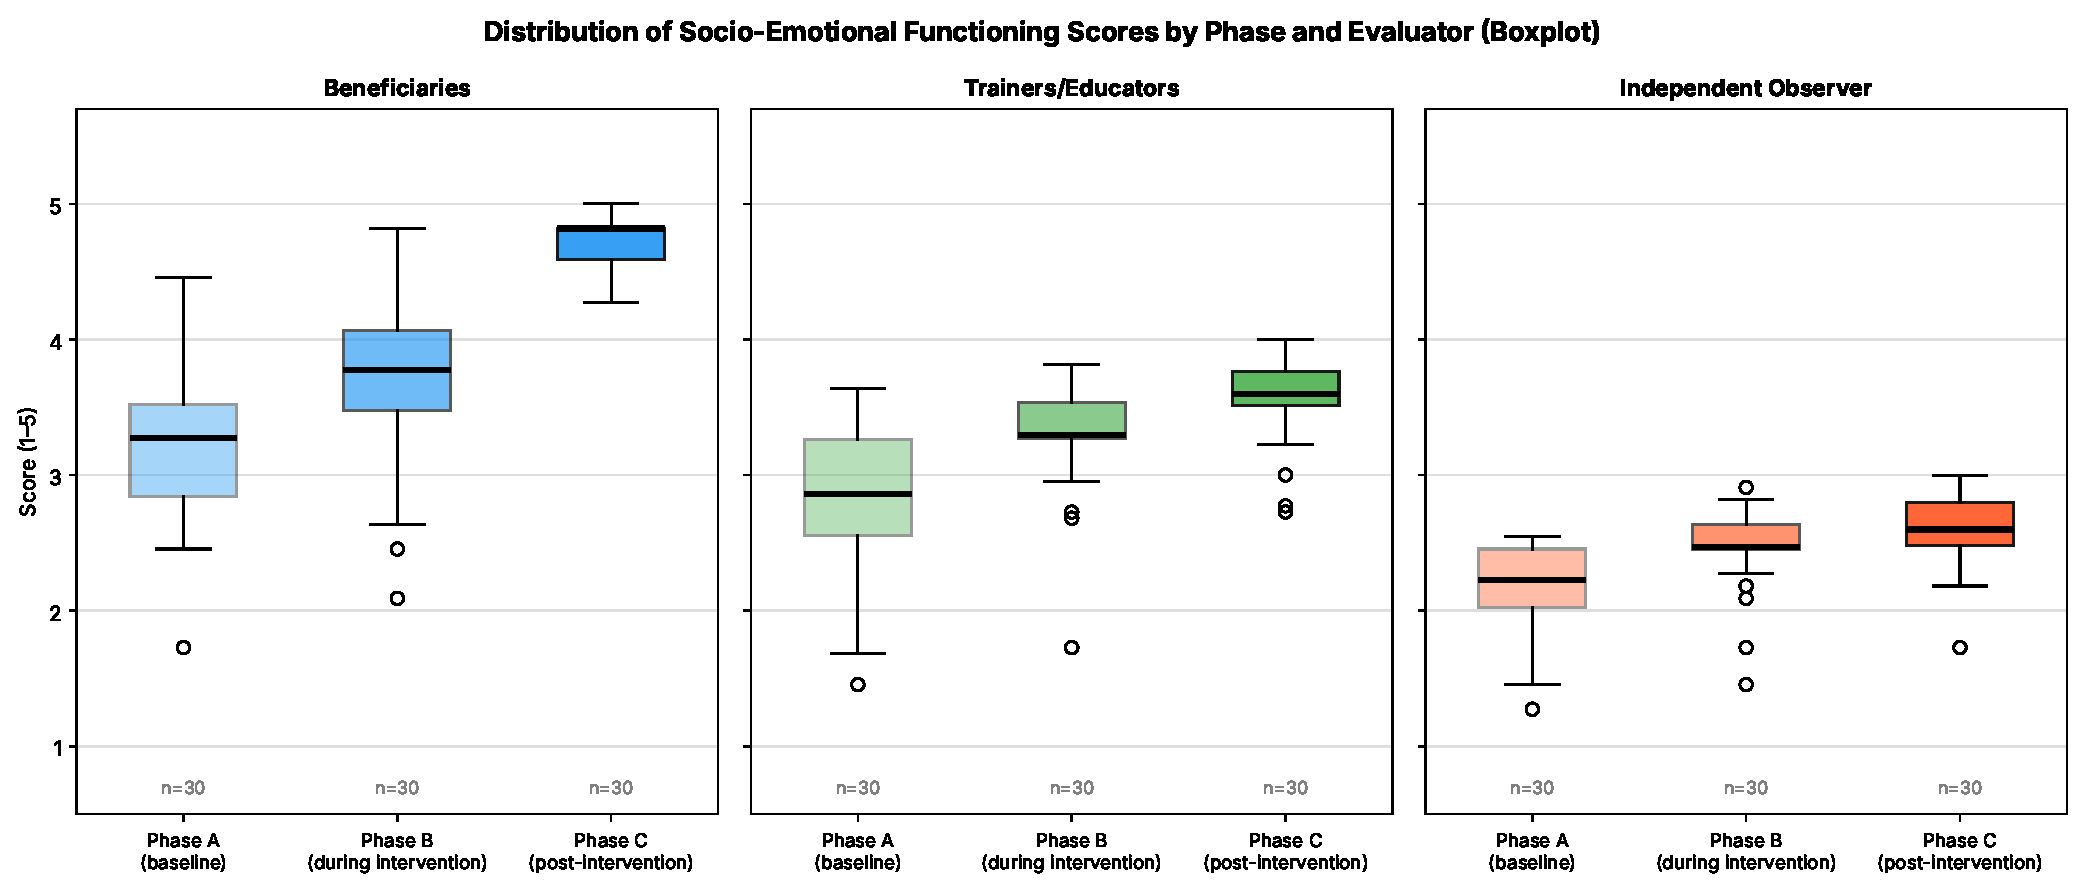
\includegraphics[width=\textwidth]{boxplot_scores.pdf}
\caption{Boxplots of socio-emotional functioning scores in Phases A, B, and C across evaluator categories.}
\label{fig:boxplot}
\end{figure}

The violin plots provide a more detailed view of score distributions across Phases A and C. Phase A was characterized by a concentration of observations around lower scores, whereas Phase C showed a clear shift toward higher values. The distribution in Phase C appeared more concentrated around positive functioning levels, suggesting that improvement was broadly distributed across participants rather than restricted to a small subgroup.

\begin{figure}[!t]
\centering
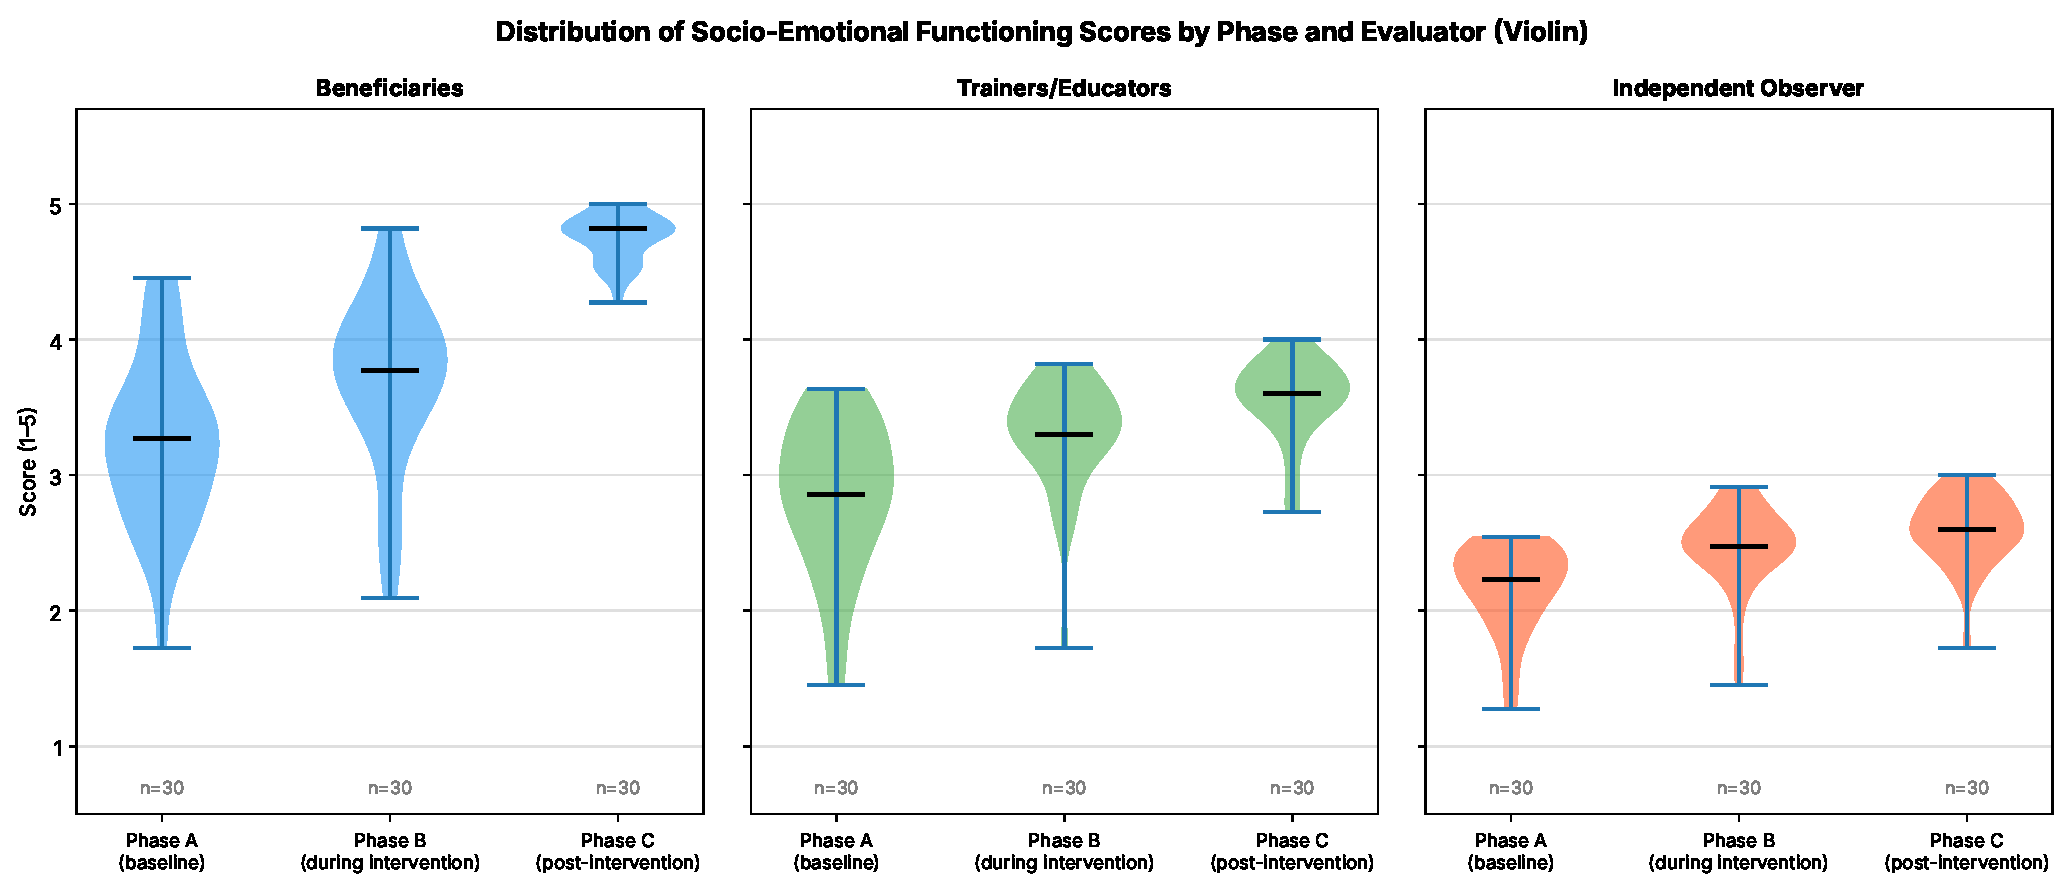
\includegraphics[width=\textwidth]{violin_scores.pdf}
\caption{Violin plots of score distributions in Phases A, B, and C.}
\label{fig:violin}
\end{figure}

\subsection{Effect Sizes and Hypothesis Testing}

The results of paired-sample $t$-tests comparing Phase A and Phase C are presented in Table~\ref{tab:paired_tests}. All evaluator categories showed statistically significant improvement from Phase A to Phase C. The largest effect was observed in beneficiary self-reports ($d=2.45$, 95\% CI [1.73, 3.16]), followed by trainer/educator ratings ($d=1.62$, 95\% CI [1.08, 2.16]) and independent observer ratings ($d=1.40$, 95\% CI [0.90, 1.91]). These values indicate large to very large effects.

\begin{table}[!t]
\caption{Paired-Sample Tests Between Phase A and Phase C and Effect Sizes}
\label{tab:paired_tests}
\centering
\begin{tabular}{lcccccc}
\hline
\textbf{Evaluator} & \textbf{Mean $\Delta$} & \textbf{$t$} & \textbf{df} & \textbf{$p$} & \textbf{Cohen's $d$} & \textbf{95\% CI for $d$} \\
\hline
Beneficiaries & +1.52 & -13.41 & 29 & $<.001$ & 2.45 & [1.73, 3.16] \\
Trainers/Educators & +0.62 & -8.88 & 29 & $<.001$ & 1.62 & [1.08, 2.16] \\
Independent observer & +0.40 & -7.69 & 29 & $<.001$ & 1.40 & [0.90, 1.91] \\
\hline
\end{tabular}
\end{table}

The corresponding forest plot is presented in Figure~\ref{fig:forest}. All effect-size estimates were positioned clearly to the right of the zero-effect line, supporting the presence of statistically significant and practically meaningful improvement across all three sources of evaluation.

\begin{figure}[!t]
\centering
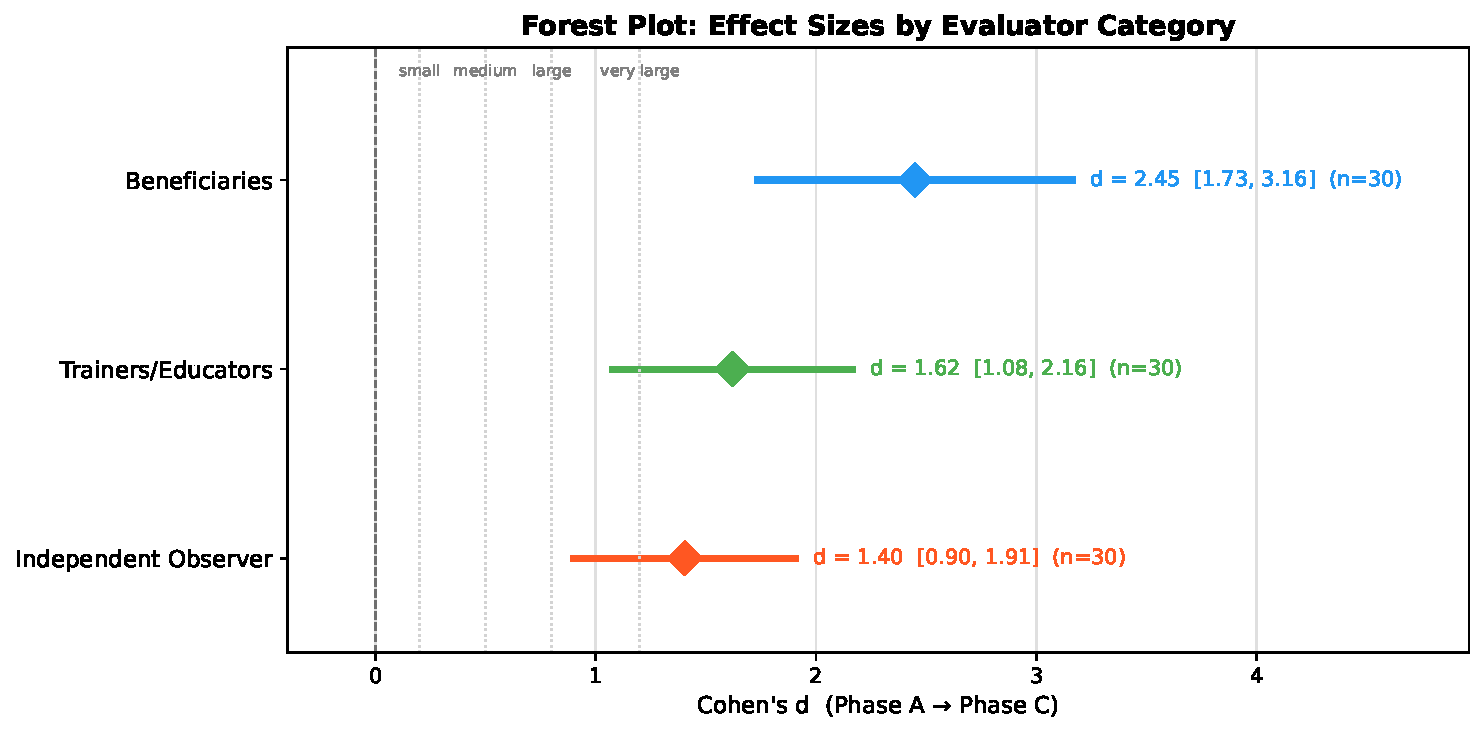
\includegraphics[width=\textwidth]{forest_effects.pdf}
\caption{Forest plot of Cohen's $d$ effect sizes across evaluator categories.}
\label{fig:forest}
\end{figure}

The Shapiro--Wilk test did not indicate a departure from normality of the Phase C $-$ Phase A difference scores for any evaluator category: beneficiaries ($W=0.945$, $p=.121$), trainers/educators ($W=0.946$, $p=.134$), and the independent observer ($W=0.953$, $p=.201$). Wilcoxon signed-rank tests, which do not rely on this assumption, led to the same conclusion in all three categories (all $p<.001$).

The Friedman test indicated statistically significant longitudinal change across the three phases for all evaluator categories: beneficiaries, $\chi^2(2)=44.86$, $p<.001$; trainers/educators, $\chi^2(2)=36.22$, $p<.001$; and independent observer, $\chi^2(2)=31.65$, $p<.001$. Pairwise comparisons using Bonferroni-corrected paired $t$-tests, with an adjusted threshold of $\alpha_{\mathrm{adj}}=.017$, showed that each phase differed significantly from the next for all evaluator categories, with all $p \leq .004$.

The very large effect size observed in beneficiary self-reports
($d = 2.45$) warrants cautious interpretation. Given the pilot
nature of the study, the small sample size ($n = 30$), and the
absence of a control condition, formal sensitivity analyses
(e.g., influence analyses or bootstrapped effect estimates) were
not conducted. The observed magnitude is likely influenced by
a combination of genuine change, ceiling effects in Phase C
($M = 4.75$, $SD = 0.18$), social desirability bias inherent
in self-report measures, and possible response-shift bias.
The convergence of findings across the two external evaluator
categories --- trainers/educators ($d = 1.62$) and the independent
observer ($d = 1.40$) --- provides partial evidence that the
improvement is not solely attributable to self-report inflation,
though it does not eliminate these alternative explanations.

\subsection{Longitudinal Trajectory}

The evolution of mean scores across the three phases is shown in Figure~\ref{fig:trajectory}. A consistent pattern of progressive improvement was observed across all evaluator categories. Beneficiaries showed the steepest upward trajectory, with a notable increase from Phase A to Phase B and further improvement from Phase B to Phase C. This suggests that the intervention began to produce measurable benefits during the early stages of implementation and that these benefits were strengthened over time.

Trainer/educator ratings also increased steadily, although in a more gradual manner. This may reflect the perspective of professionals who observe beneficiaries in daily routines and tend to provide more conservative evaluations of behavioral change. The independent observer showed a similar positive trajectory, further supporting the objectivity and consistency of the findings.

\begin{figure}[!t]
\centering
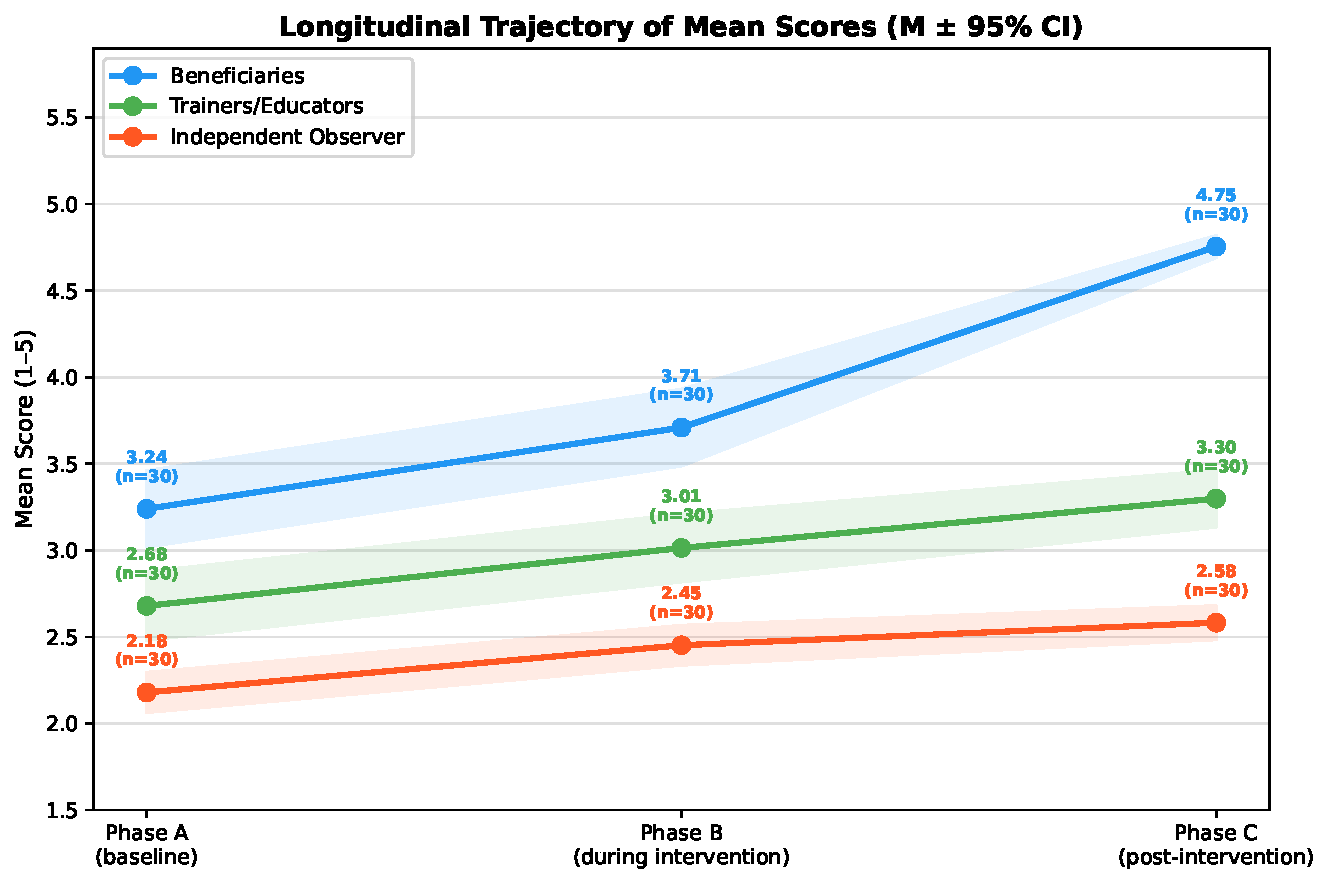
\includegraphics[width=\textwidth]{trajectory_scores.pdf}
\caption{Longitudinal trajectory of mean scores across Phases A, B, and C.}
\label{fig:trajectory}
\end{figure}

Overall, the results indicate that the intervention was associated with significant improvement in emotion recognition, cooperation, group participation, and broader socio-emotional functioning. The convergence of findings across beneficiaries, trainers/educators, and the independent observer provides cross-source support for the effectiveness of the experiential socio-emotional intervention in a DCC setting.


\section{Discussion}

The findings of the present study indicate that the structured experiential socio-emotional intervention was associated with statistically significant and practically meaningful improvements in the socio-emotional functioning of adult beneficiaries attending the Day Care Center. The steady increase in mean scores across all three measurement phases, together with the large effect sizes observed across evaluator groups, indicates that ratings of emotional recognition, cooperation, expression, group participation, and positive interpersonal interaction rose markedly over the course of the program; whether this change is attributable to the program itself cannot be established with the present design.

The marked improvement reported by beneficiaries themselves ($d = 2.45$) is consistent with previous studies showing that participation in stable, safe, and structured group activities may enhance self-perception, confidence, and social engagement among adults with disabilities \parencite{hall2009}. The increase in self-reported functioning may reflect greater self-awareness and a more positive internal experience, both of which are central dimensions of emotional intelligence as conceptualized by \textcite{goleman1995}.

Trainers and educators also reported significant improvement ($d = 1.62$), with a pattern of change broadly parallel to that observed in self-reports. Although professionals often evaluate functioning more conservatively due to continuous exposure to everyday behavioral challenges, the convergence in trajectories strengthens confidence in the consistency of the findings.

Importantly, the independent observer, who had no prior relational involvement with participants, also identified substantial gains ($d = 1.40$). Agreement across the three sources of evaluation represents one of the strongest methodological contributions of the present study. In disability research, ratings may be influenced by familiarity effects, expectancy bias, or relational dynamics. Therefore, cross-source convergence enhances internal validity and reduces the likelihood that the findings merely reflect rater-specific perceptions.

From a theoretical perspective, the findings align closely with the framework of SEL. CASEL emphasizes that competencies such as self-awareness, self-management, empathy, relationship skills, and responsible decision-making are strengthened through repeated participation in structured and emotionally supportive learning environments \parencite{casel2020,weissberg2015}. The intervention implemented in the present study was explicitly designed around these principles, suggesting that SEL-informed approaches may also be highly relevant beyond school settings and into adult disability services.

The results are also consistent with group-process theory. Yalom and Leszcz argue that therapeutic factors such as universality, interpersonal learning, group cohesion, emotional catharsis, and hope are central mechanisms of change in group contexts \parencite{yalom2005}. The repeated small-group format of the intervention likely facilitated these processes. Participants were given opportunities to share experiences, express emotions, collaborate creatively, and experience belonging within a psychologically safe collective environment.

In addition, the findings support growing evidence suggesting that arts-based interventions can function as powerful vehicles for socio-emotional development, particularly among populations with communication, cognitive, or psychosocial support needs \parencite{stickley2018,leavy2015}. The program ``The Universe Within Us'' combined theatre, music, movement, symbolic creation, and narrative dialogue. Such multimodal methods may be especially effective because they enable expression beyond purely verbal communication, allowing embodied, symbolic, and relational forms of meaning-making.

Transformative learning theory may also help interpret the findings. \textcite{mezirow2000} proposed that emotionally meaningful experiences can stimulate perspective transformation and personal growth. The strong participant engagement observed during the intervention suggests that creative and emotionally resonant experiences may have facilitated reflection, identity development, and new patterns of social participation.

From a developmental standpoint, the results also resonate with Vygotsky's socio-cultural theory, according to which learning emerges through guided participation and social interaction \parencite{vygotsky1978}. As participants became more familiar with the structure and expectations of the program, they may have increasingly benefited from scaffolded participation within their zone of proximal development. This may explain the progressive gains observed across phases rather than a short-term isolated improvement.

Another plausible mechanism concerns belongingness and social identity. Group membership and positive shared identity have been shown to improve well-being and resilience through what has been described as the ``social cure'' process \parencite{haslam2018}. In the present intervention, participants repeatedly engaged in collaborative creative experiences, public performance, and shared symbolic production, all of which may have strengthened identity, cohesion, and perceived social value.

The magnitude of change observed in the present study appears larger than that reported in many previous interventions targeting social skills or participation in adults with disabilities, where small-to-moderate effects are more common \parencite{giummarra2022}. One possible interpretation, which the present design cannot test, is that holistic interventions combining emotional safety, experiential learning, creative expression, and stable group processes act jointly rather than through any single component; alternative explanations, including measurement reactivity and the absence of a comparison condition, remain equally plausible.

The findings may also be interpreted within the Quality of Life framework proposed for persons with intellectual disabilities. Schalock and colleagues identify emotional well-being, interpersonal relations, self-determination, social inclusion, and personal development as central quality-of-life domains \parencite{schalock2010}. Improvements in emotional expression, cooperation, group belonging, and active participation suggest that the intervention may have contributed not only to isolated competencies but to broader psychosocial quality-of-life dimensions.

Similarly, supported participation in community and relational contexts has been identified as a key pathway to inclusion \parencite{bigby2015}. The public performance component of the intervention, involving schools and the local community, may have strengthened visibility, dignity, and reciprocal social recognition, extending the impact beyond the internal group setting.

The present study was conducted within a specific cultural and
institutional context. While this context is representative of
community-based disability services in Southern Europe, caution
is warranted when generalizing findings to other national systems.
DCCs in different countries may vary considerably in terms of
staffing ratios, program duration, participant characteristics,
and available resources. Nevertheless, the core principles underlying
the intervention --- experiential learning, group cohesion,
arts-based expression, and structured emotional safety --- are not
context-specific and have been documented as effective across diverse
service settings internationally \parencite{giummarra2022,leavy2015}.
Future replications in different national and cultural contexts
would strengthen the external validity of these findings.

\subsection{Limitations}

Despite the strength and consistency of the findings, several limitations should be acknowledged. First, the study was conducted in a single Day Care Center without a control group. Consequently, causal attribution should be made cautiously, as maturation effects, seasonal influences, or Hawthorne effects cannot be excluded.

Second, the very large effect sizes, particularly in beneficiary self-reports, should be interpreted conservatively. Possible inflating factors include social desirability bias, ceiling effects in the final phase, expectancy effects, response-shift bias, and regression to the mean.

Third, although the instrument demonstrated satisfactory internal consistency, it has not yet undergone full psychometric validation (e.g., factor structure, convergent validity, discriminant validity). Fourth, the sample size, while adequate for within-subject analyses, remains modest for subgroup comparisons or moderator analyses.

Fifth, inter-rater reliability between the two trainers/educators is not reported in this article. The mean of their scores was used as a composite rating, and the precision of the trainer-based evaluation component should therefore be regarded as uncertain. Moreover, 63 of the 358 individual ratings (17.6\%; 23.5\% of the 268 trainer and observer ratings) were not contained in the electronic export of the rating platform and were supplied subsequently by the facility; the circumstances of their original recording could not be independently verified.

Sixth, the sample was heterogeneous with respect to primary diagnosis, and the modest sample size precluded subgroup analyses comparing participants with and without a documented intellectual disability, or by severity of intellectual disability. The findings should therefore be interpreted as applying to the mixed population served by adult day care services rather than to intellectual disability specifically. In addition, no standardized measure of cognitive or adaptive functioning was administered, so the influence of baseline functioning on the observed change could not be examined.

Finally, intervention fidelity was not formally measured through observational checklists or adherence protocols, which limits precision regarding replicability across settings.

\subsection{Future Directions}

Future research may strengthen the evidence base in several ways. Replication across multiple Day Care Centers or similar disability-service settings would improve external validity. Randomized or quasi-experimental designs with comparison groups would allow stronger causal inference.

Long-term follow-up assessments are also needed to determine whether gains are sustained after program completion. Future studies may further integrate physiological indicators of emotional regulation, such as heart-rate variability or stress biomarkers, to complement behavioral outcomes.

In addition, mixed-methods designs incorporating qualitative interviews with beneficiaries, families, and staff could offer deeper insight into lived experience and mechanisms of change. Finally, future psychometric validation of the assessment instrument would support broader use in disability-service evaluation and intervention research. Specifically, exploratory and confirmatory factor analyses should be conducted to examine the factor structure of the instrument, while test-retest reliability studies would provide evidence of measurement stability over time.


\section{Conclusion}

The present study provides preliminary but consistent evidence that a holistic and experiential socio-emotional empowerment program may produce notable and promising improvements in the emotional and social functioning of adults with disabilities within a day care setting. The consistent upward trajectory of scores across the three evaluation phases, combined with large effect sizes and substantial agreement among beneficiaries, trainers, and an independent observer, suggests that the intervention was associated with improvements through mechanisms of experiential learning, group cohesion, relational support, and guided emotional expression.

The findings are consistent with contemporary theoretical frameworks of SEL, emotional intelligence, and socio-cultural learning theory. They support the view that adults with disabilities are capable of developing and strengthening complex psychosocial competencies when they participate in structured, emotionally safe, and socially meaningful environments.

The contribution of the present study is twofold. First, it offers an empirically informed intervention model that may be adapted and replicated in other Day Care Centers and community-based disability services. Second, it enriches the international literature with evidence from a field in which rigorous empirical research remains comparatively limited, particularly regarding adult populations in non-institutional support settings.

Methodologically, the study demonstrates the value of combining longitudinal multi-phase assessment with multiple evaluator perspectives. The convergence of findings across self-reports, professional ratings, and independent observation strengthens confidence in the robustness of the results and offers a useful framework for future applied evaluation studies.

The practical implications are also noteworthy. Services supporting adults with disabilities may benefit from integrating programs that cultivate emotional awareness, interpersonal connection, cooperative participation, and creative expression. Such interventions may function not only as educational tools, but also as pathways to empowerment, autonomy, psychological well-being, and community inclusion.

The findings also align with broader policy directions, including the European Disability Rights Strategy 2021--2030, which promotes community-based models of care that enhance participation, independence, dignity, and equal opportunities.

Overall, the present study highlights that adults with disabilities possess substantial developmental potential when provided with appropriate structure, sustained support, and meaningful opportunities for learning and participation. Investing in such environments is therefore not merely a service innovation, but a matter of social justice, human development, and inclusive citizenship.


% ---------------------------------------------------------------
\section*{Author Contributions}
Author contributions are provided on the separate title page (blinded for double-anonymous peer review).

% REQUIRED STATEMENTS
% ---------------------------------------------------------------

\section*{Conflict of Interest Disclosure}
Three of the four authors are affiliated with the Day Care Center in which the study was conducted, as described in the Researcher Positionality section. The authors declare no financial conflict of interest.

\section*{Ethics Approval Statement}
The study was reviewed and approved by the administration of the Day Care Center in which it was conducted [name blinded for review] on 1 October 2025. As the study constituted an evaluation of a program forming part of the facility's regular provision rather than an experimental clinical intervention, review by an external research ethics committee was not required under applicable national guidelines. The study was conducted in accordance with the ethical principles of the Declaration of Helsinki. All participants, or their legal guardians where applicable, were informed about the purpose of the evaluation and provided voluntary consent prior to inclusion. Participant anonymity and confidentiality were maintained throughout, and all data were pseudonymized prior to analysis.

\section*{Data Availability Statement}
The pseudonymized analysis dataset and all analysis code are publicly available at a GitHub repository (URL blinded for review; see title page). The raw questionnaire export, which contains participant identifiers, is not shared.

\section*{Funding Statement}
This research received no external grant funding. The study was conducted with
the institutional support of the Day Care Center [name blinded for review],
which provided the research setting, access to participants, and staff time
throughout the implementation and evaluation of the program.

\section*{Acknowledgements}
% Acknowledgements blinded for double-anonymous review.
% Restore acknowledgments at revision/acceptance stage.

\printbibliography

\end{document}
